\documentclass[a4paper,12pt]{report}
\usepackage[utf8]{vietnam}
\usepackage{}
\usepackage{graphicx}
\usepackage{fancybox}
\usepackage{longtable}
\usepackage{listings}
\usepackage{relsize}
\usepackage{cases} 
\usepackage[left=3cm, right=2.00cm, top=2.00cm, bottom=2.00cm]{geometry}
\lstset{
   %keywords={break,case,catch,continue,else,elseif,end,for,function,
   %   global,if,otherwise,persistent,return,switch,try,while},
   basicstyle=\ttfamily \fontsize{12}{15}\selectfont,   
	% numbers=left,
   frame=lrtb,
tabsize=2
}
\setlength{\parskip}{0.6em}
\usepackage{hyperref}
\usepackage{float}
\hypersetup{
    colorlinks,
    citecolor=black,
    filecolor=black,
    linkcolor=black,
    urlcolor=black
}
\usepackage[nottoc]{tocbibind}
\usepackage[english]{babel}
\usepackage{indentfirst}
\addto\captionsenglish{%
 \renewcommand\chaptername{Phần}
 \renewcommand{\contentsname}{Mục lục} 
 \renewcommand{\listtablename}{Danh sách bảng}
 \renewcommand{\listfigurename}{Danh sách hình vẽ}
 \renewcommand{\tablename}{Bảng}
 \renewcommand{\figurename}{Hình}
 \renewcommand{\bibname}{Tài liệu tham khảo}
}
\begin{document}
\thispagestyle{empty}
\thisfancypage{
\setlength{\fboxrule}{1pt}
\doublebox}{}
\begin{center}
{\fontsize{16}{19}\fontfamily{cmr}\selectfont TRƯỜNG ĐẠI HỌC BÁCH KHOA HÀ NỘI\\
VIỆN CÔNG NGHỆ THÔNG TIN VÀ TRUYỀN THÔNG}\\
\textbf{------------*******---------------}\\[1cm]

\includegraphics[scale=0.13]{hust.jpg}\\[1.3cm]

{\fontsize{32}{43}\fontfamily{cmr}\selectfont BÁO CÁO}\\[0.1cm]
{\fontsize{38}{45}\fontfamily{cmr}\fontseries{b}\selectfont MÔN HỌC}\\[0.2cm]
{\fontsize{19}{20}\fontfamily{phv}\selectfont Tính toán khoa học }\\[0.2cm]
{\fontsize{13}{20}\fontfamily{cmr}\selectfont Đề tài: Mạng Google Inception trong bài toán phân loại}\\[2.5cm]
\end{center}
\hspace{1cm}\fontsize{14}{16}\fontfamily{cmr}\selectfont \textbf{Nhóm sinh viên thực hiện:}

\begin{longtable}{l c c}

Họ và tên & MSSV  & Lớp\\
Nguyễn Tuấn Đạt & 20130856 & CNTT2.02-K58 \\
Đặng Quang Trung & 20134145 & CNTT2.02-K58 \\
Phan Anh Tú & 20134501 & CNTT2.01-K58 \\
\end{longtable}

\hspace{0.6cm}\fontsize{14}{16}\fontfamily{cmr}\selectfont \textbf{Giảng viên môn học: }TS. Đinh Viết Sang \\[1.5cm]
\begin{center}
\fontsize{16}{19}\fontfamily{cmr}\selectfont Hà Nội 1--2017

\end{center}
\newpage

\pdfbookmark{\contentsname}{toc}
\tableofcontents
\listoffigures


\phantomsection
\addcontentsline{toc}{chapter}{Lời cảm ơn}
\chapter*{Lời cảm ơn}
Chúng em xin chân thành cảm ơn Thầy giáo, TS. Đinh Viết Sang đã tận tình giảng dạy, hướng dẫn chúng em thực hiện đề tài này. Trong quá trình thực hiện, đề tài của chúng em không tránh khỏi những hạn chế, thiếu sót, chúng em rất mong nhận được những ý kiến đánh giá, nhận xét của Thầy để đề tài này có thể được hoàn thiện hơn.


\chapter{Đặt vấn đề}
Trong bối cảnh nghành công nghiệp công nghệ thông tin đang phát triển rất mạnh mẽ ngày này, có lẽ Deep Learning là một trong những từ khóa được quan tâm nhất. Deep Learning đang được ứng dụng ngày càng rộng rãi trong các công việc của cuộc sống hàng ngày như: ô tô tự lái, nhận diện giọng nói, nhận diện khuôn mặt ....
\par Là một sinh viên ngành khoa học máy tính, chúng em nhận thấy cần trang bị những kiến thức cần thiết về Deep Learning. Vì vậy, mục tiêu của bài tập lớn này của chúng em là tìm hiểu về Deep Learning và cụ thể là tìm hiểu về mạng Google Inception trong bài toán phân loại.
\par Google Inception hay  GoogleNet là mạng biến thể của mạng Convolutional neural network (A deep convolutional neural network architecture \cite{googlenet}). Convolutional neural network (CNN) là một dạng của mạng neuron nhân tạo thông thường (Artificial neural network - ANN) (những mạng này sẽ được chúng em giới thiệu ở phần sau của báo cáo).  
\par Phần tiếp theo của báo cáo bao gồm các phần sau: phần 1 và phần 2 giới thiệu về mạng ANN, CNN; các phần tiếp theo sẽ trình bày về mạng Google Inception và các cải tiến của nó. Cụ thể:
\par \textbf{Phần 1}
\par \textbf{Phần 2} 

\chapter{Giới thiệu mạng neural nhân tạo (ANN)}

\chapter{Giới thiệu mạng CNN}
\section{Kiến trúc tổng quan của CNN}
Giống như các mạng neuron thông thường khác đã được giới thiệu phần trước, Nó nhận được đầu vào và biến đổi nó thông qua một loạt các lớp ẩn. Mỗi lớp ẩn được tạo thành từ một tập các neuron, trong đó mỗi một neuron được kết nối đầy đủ trong các lớp trước đó, và ở các neuron trong lớp đơn hoàn toàn không phụ thuộc nhau và không chia sẻ bất kì kết nối nào. Lớp cuối cùng kết nối đầy đủ được gọi ở lớp đầu ra và trong cài đặt phân lớp nó đại diện cho điểm của mỗi lớp.
\begin{figure}[H]
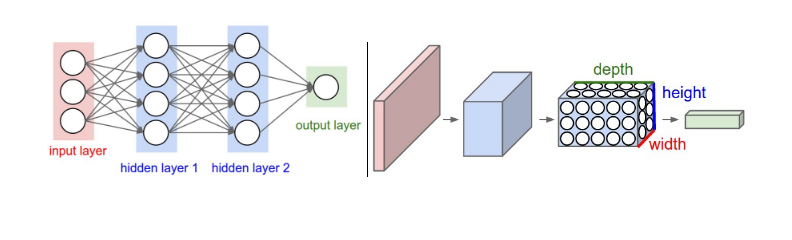
\includegraphics[scale=0.7]{img1.png}
\caption{Mô hình tổng quan CNN}
\end{figure}
\section{Các lớp sử dụng để xây dựng ConvNets}
Như đã mô tả ở trên, một ConvNet đơn giản là một chuỗi các lớp, và mỗi lớp của một ConvNet chuyển một khối lượng kích hoạt khác thông qua một hàm khả vi. Có 3 lớp chính để xây dựng kiến trúc ConvNet: Convolutional Layer, Pooling Layer, và Fully-Connected Layer. Sắp xếp các lớp này để tạo thành một kiến trúc ConvNet.ConvNet có một vài biến thể khác:
\begin{itemize}
\item[•] Một kiến trúc ConvNet là trong trường hợp đơn giản là một danh sách các lớp mà đổi khối lượng hình ảnh thành một khối lượng đầu ra (ví dụ như tổ chức các điểm lớp).
\item[•] Có một vài loại riêng biệt của lớp (ví dụ như CONV / FC / RELU / POOL là bởi đến nay phổ biến nhất).
\item[•] Mỗi lớp chấp nhận một khối lượng 3D đầu vào và biến đổi nó vào một đầu ra khối lượng 3D thông qua một hàm khả vi
\item[•] Mỗi lớp có thể có hoặc không có thông số (ví dụ CONV / FC làm, RELU / POOL không)
\item[•] Mỗi lớp có thể có hoặc có thể không có siêu tham bổ sung (ví dụ như CONV / FC / POOL làm, RELU không).
\end{itemize}
\section{Convolution Layer}
Convolution Layer là khối xây dựng cốt lõi của mạng CNN \\ 

\textbf{Tổng quan:} Thông số lớp CONV của bao gồm một tập hợp các bộ lọc học. Mỗi bộ lọc là nhỏ không gian (cùng chiều rộng và chiều cao), nhưng kéo dài qua toàn bộ chiều sâu của khối lượng đầu vào. Mỗi một bộ lọc sẽ trượt trên toàn chiều rộng và chiều cao của khối lượng đầu vào và tính toán các sản xuất nhân giữa các mục của bộ lọc và các đầu vào tại vị trí bất kỳ. Chúng ta trượt bộ lọc trên chiều rộng và chiều cao của khối lượng đầu vào, chúng tôi sẽ tạo ra một ánh xạ kích hoạt 2 chiều cung cấp cho các phản ứng của bộ lọc đó ở mọi vị trí không gian. \\ 

\textbf{Quan điểm não:}Mỗi mục trong khối lượng đầu ra 3D cũng có thể được hiểu như là một sản phẩm của một tế bào thần kinh mà nhìn vào chỉ một vùng nhỏ trong các tham số đầu vào và chia sẻ với tất cả các tế bào thần kinh bên trái và đúng không gian \\ 
 
\textbf{Kết nối địa phương:} Khi làm việc với các đầu vào chiều cao như hình ảnh, như chúng ta đã thấy ở trên nó là không thực tế để kết nối các nơron cho tất cả các tế bào thần kinh trong khối lượng trước đó.  Thay vào đó, chúng ta sẽ kết nối từng tế bào thần kinh để chỉ một khu vực địa phương của khối lượng đầu vào. Phạm vi không gian của kết nối này là một siêu tham số gọi là khu vực tiếp nhận( bằng với kích cỡ của bô lọc ). Mức độ kết nối dọc theo trục sâu luôn bằng chiều sâu của khối lượng đầu vào. Điều quan trọng cần nhấn mạnh một lần nữa không đối xứng này trong cách chúng ta đối xử với các chiều không gian (chiều rộng và chiều cao) và chiều sâu là: Các kết nối được địa phương trong không gian (cùng chiều rộng và chiều cao), nhưng luôn luôn đầy đủ dọc theo toàn bộ chiều sâu của khối lượng đầu vào.
\begin{figure}[H]
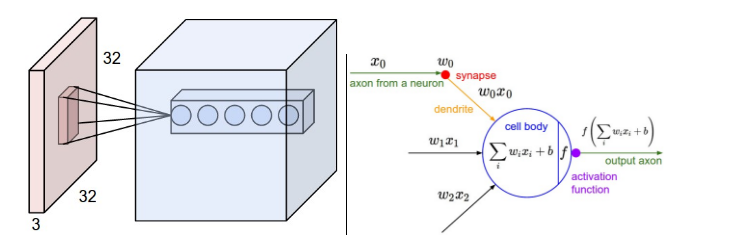
\includegraphics[scale=0.7]{img2.png}
\caption{CONV Layer}
\end{figure}
\textbf{Sắp xếp không gian:} Không gian số lượng các neurons ở đầu ra của mỗi khối làm thế nào để sắp xếp chúng. Ở đây có 3 siêu tham số dùng để kiểm soát kích thước của khối lượng đầu ra:depth(độ sâu), stride(sải chân) vào đệm (zero-padding):
\begin{itemize}
\item[1. ] Thứ nhất, độ sâu của khối lượng đầu ra là một hyperparameter: nó tương ứng với số lượng bộ lọc chúng tôi muốn sử dụng, mỗi học tập để tìm kiếm một cái gì đó khác nhau trong các đầu vào.
\item[2. ] Thứ hai, chúng ta phải xác định các stride mà chúng ta trượt lọc. Khi stride là 1 sau đó chúng tôi di chuyển các bộ lọc một điểm ảnh tại một thời điểm. Khi stride là 2 (hoặc khác thường 3 hoặc nhiều hơn, mặc dù điều này là hiếm trong thực tế) sau đó các bộ lọc nhảy 2 điểm ảnh tại một thời điểm khi chúng ta đẩy chúng xung quanh. Điều này sẽ tạo ra khối lượng sản lượng nhỏ không gian.
\item[3. ] Thứ ba, đôi khi để thuân tiện hơn để lề bao quanh ngoài của ảnh với số không. Các kích thước này zero-padding là một hyperparameter. Điểm hay của zero-padding là nó sẽ cho phép chúng ta kiểm soát kích thước không gian của khối lượng đầu ra (thường gặp nhất như chúng ta sẽ thấy sớm, chúng ta sẽ sử dụng nó để bảo toàn chính xác kích thước không gian của khối lượng đầu vào để các đầu vào và đầu ra rộng và chiều cao đều giống nhau).
\end{itemize} 

\textbf{Tham số không gian:} Nó chỉ ra rằng chúng ta có thể làm giảm đáng kể số lượng các thông số bằng cách làm cho một giả định hợp lý: đó, nếu một tính năng rất hữu ích để tính toán tại một số vị trí không gian (x, y), sau đó nó nên cũng có ích để tính toán tại một vị trí khác nhau (x2 , y2). Nói cách khác, biểu thị một lát 2 chiều duy nhất của chiều sâu như một lát độ sâu. Trong thực tế trong quá trình lan truyền ngược, mỗi tế bào thần kinh trong khối lượng sẽ tính toán gradient cho trọng lượng của nó, nhưng các gradients sẽ được thêm lên trên mỗi miếng chiều sâu và chỉ cập nhật một bộ trọng lượng mỗi slice. \\
 
\textbf{Tóm lại:}Lớp Conv Layer
\begin{itemize}
\item Đầu vào một khối lượng kích thước $W_1*H_1*D_1$.
\item Yêu cầu 4 siêu tham số:
\begin{itemize}
\item Số bộ lọc K,
\item Kích cỡ mỗi bộ lọc F,
\item Bước sải S,
\item Số lương của lề (zeros-padding) P
\end{itemize}
\item Tạo ra 1 khối có kích cỡ $W_2*H_2*D_2$
\begin{itemize}
\item $W_2= \frac{(W_2 - F + 2P)}{S} + 1$
\item $H_2=\frac{(H_1 - F + 2P)}{S}+1$(chiều cao và chiều rộng tính như nhau bởi đối xứng).
\item $D_2 = K$.
\item Với chia sẻ tham số,$F*F*D_1$ trọng số/mỗi bộ lọc. Tổng trọng số là $(F*F*D_1)*K$ và K là biases.
\item Trong khối lượng đầu ra,độ sâu lát thứ d(kích cỡ $W_2*H_2$) là kết quả của việc thực hiện một chập hợp lệ của bộ lọc thứ d với đầu vào có sải là S,và sau đó bù lại bởi bias thứ d.
\end{itemize}
\end{itemize}
Một cài đặt thông thường các siêu tham só là $F = 3, S = 1, P= 1 $. Tuy nhiên, có những quy ước chung và quy tắc vận dụng mà thúc đẩy các siêu tham
\begin{center}
\begin{figure}[H]
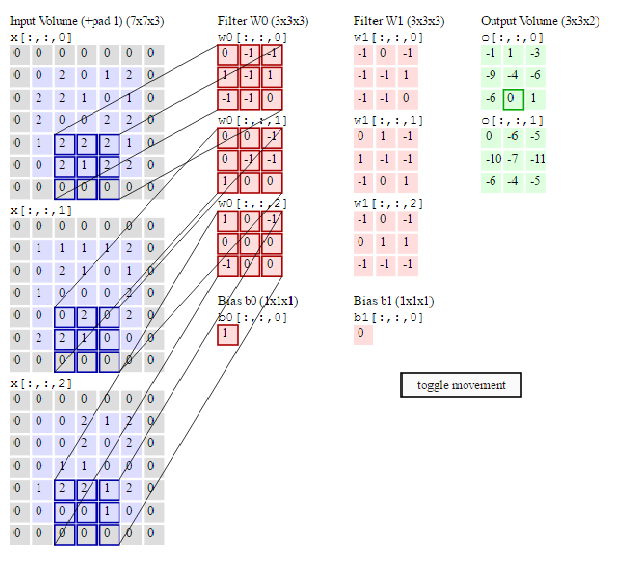
\includegraphics[scale=0.7]{img3.png}
\caption{Ví dụ CONV}
\end{figure}
\end{center}
\section{Pooling Layer}
Nó được phổ biến định kỳ thêm một layer Pooling ở giữa lớp Conv liên tiếp trong một kiến trúc ConvNet. Chức năng của nó là để dần dần làm giảm kích thước không gian của các đại diện để giảm số lượng các thông số và tính toán trong mạng, và vì thế để kiểm soát cũng overfitting. Các Pooling lớp hoạt động độc lập trên mỗi lát chiều sâu của đầu vào và thay đổi kích thước nó về không gian, sử dụng các hoạt động MAX. Các hình thức phổ biến nhất là một lớp tổng hợp với các bộ lọc kích thước $2*2$ áp dụng với một sải chân của 2 downsamples mỗi lát sâu trong đầu vào của 2 dọc theo cả hai chiều rộng và chiều cao,loại bỏ $75\%$ các kích hoạt.Mỗi hoạt động MAX sẽ trong trường hợp này là dùng một tối đa hơn 4 số (vùng $2*2$ ít trong một số lát chiều sâu). Chiều sâu vẫn không thay đổi. Tổng quát hơn, các lớp tổng hợp:
\begin{itemize}
\item Đầu vào là các khối kích thước $W_1*H_1*D_1$.
\item Yêu cầu 2 tham số
\begin{itemize}
\item Phạm vi không gian(F)
\item Các bước tiến(S)
\end{itemize}
\item Sản xuất một khối lượng kích thước $W_2*H_2*D_2$ ở đây:
\begin{itemize}
\item $W_2 =\frac{(W_1 - F)}{S} + 1$
\item $H_2 =\frac{(H_1 - F)}{S} + 1$
\item $D_2 = D_1$
\end{itemize}
\item Tham số zeros-padding khi nó tính một hàm cố định của các đầu vào
\item Lưu ý rằng nó không phải là phổ biến để sử dụng zero-đệm cho việc kết hợp các lớp
\end{itemize}
\begin{center}
\begin{figure}[H]
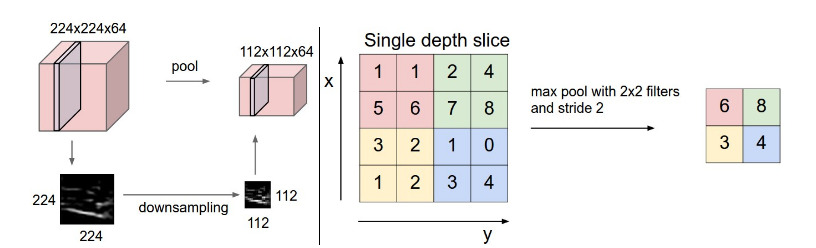
\includegraphics[scale=0.8]{img4.png}
\caption{Ví dụ CONV}
\end{figure}
\end{center}
\section{Fully-connected Layer(kết nối đầy đủ)}
Tế bào thần kinh trong một lớp đầy đủ kết nối có các kết nối đầy đủ với tất cả các kích hoạt trong lớp trước, như đã thấy trong thường xuyên Neural Networks. Kích hoạt của họ do đó có thể được tính toán với một phép nhân ma trận theo sau là một xu hướng bù đắp. Xem các Neural Network phần của các ghi chú để biết thêm thông tin.
\section{Các lớp mẫu của mô hình về CNN}
Các hình thức phổ biến nhất của một kiến trúc ConvNet xếp một vài lớp CONV-RELU, sau đó với lớp POOL, và lặp đi lặp lại mô hình này cho đến khi hình ảnh đã được sáp nhập về không gian đến một kích thước nhỏ. Tại một số điểm, nó được phổ biến để chuyển đổi sang lớp kết nối đầy đủ. Các lớp kết nối đầy đủ cuối cùng nắm giữ đầu ra, chẳng hạn như điểm số lớp. Nói cách khác, kiến trúc ConvNet phổ biến nhất theo mẫu sau: \\
\\
\small{
\textbf{INPUT -> [[CONV -> RELU]*N -> POOL?]*M -> [FC -> RELU]*K -> FC}
}
\\ \\
Ở đây * chỉ ra sự lặp lại, và POOL? chỉ ra một lớp tổng hợp tùy chọn. Hơn nữa, N >= 0(và thường N <= 3), M >= 0, K >= 0(và thường K < 3)s
Trong phần này chúng em sẽ trình bày về kiến trúc của mạng Google Inception (GoogleNet), nhưng trước hết trong phần đầu tiên chúng em sẽ giới thiệu tổng quan về mạng GoogleNet, mục đích khi thiết kế mạng, những ưu điểm của nó so với các mạng khác trong bài toán phân loại.

\section{Tổng quan về GoogleNet}
Inception là một biến thể của mạng CNN (a deep convolutional neural network architecture \cite{googlenet}), một trong những khác biệt lớn nhất của kiến trúc này là sự cải thiện của tài nguyên tính toán bên trong mạng (mặc dù mạng tăng cả về chiều sâu (số lượng tầng trong mạng) và chiều rộng (số lượng neural trong một tầng) nhưng chi phí tính toán vẫn không đổi (chi phí để học các trọng số trong mạng)) (Mạng GoogleNet trong ILSVRC 2014 (ImageNet Large-Scale Visual Recognition Challenge) có số lượng tham số ít hơn 12 lần với kiến trúc mạng đã chiến thắng năm 2012). 


\section{Inception Module}	



\begin{thebibliography}{9}
\bibitem{googlenet} C. Szegedy, W. Liu, Y. Jia, P. Sermanet, S. Reed, D. Anguelov, D. Erhan, V. Vanhoucke, and A. Rabinovich. \textit{Going deeper with convolutions}

\bibitem{rethinking} C. Szegedy, V. Vanhoucke, S. Ioffe, J. Shlens, and Z. Wojna. \textit{Rethinking the inception architecture for computer vision}

\bibitem{inceptionv4} C. Szegedy, S. Ioffe, and V. Vanhoucke. \textit{Inception-v4, Inception-ResNet and the Impact of Residual Connections on Learning}

\end{thebibliography}

\end{document}
